\documentclass{article}[18pt]
\usepackage[utf8]{inputenc}
\usepackage[margin=0.7in]{geometry}
\usepackage{parselines} 
\usepackage{amsmath}
\usepackage{titlesec}
\usepackage{pgfplots}
\usepackage{graphicx}
\usepackage[english]{babel}
\usepackage{fancyhdr}
\usepackage{gensymb}
\usepackage{enumerate}
\usepackage{amssymb}
\pgfplotsset{width=10cm,compat=1.9}
\usepackage{tikz}
\usetikzlibrary{calc,shapes.geometric, arrows}
\titlespacing\section{0pt}{14pt plus 4pt minus 2pt}{0pt plus 2pt minus 2pt}
\newlength\tindent
\setlength{\tindent}{\parindent}
\setlength{\parindent}{0pt}
\renewcommand{\indent}{\hspace*{\tindent}}	
\newcommand{\cred}[1]{\color{red}#1}
\newcommand{\cblue}[1]{\color{blue}#1}
\newcommand{\cgreen}[1]{\color{green}#1}
\hyphenpenalty=10000
\pagestyle{fancy}
\fancyhf{}
\rhead{Sam Robbins 13SE}
\lhead{A Level Maths - D2}
\rfoot{Page \thepage}
\usepackage{float}

\newcommand{\tikzmark}[1]{\tikz[overlay,remember picture] \node (#1) {};}

\newcommand{\DrawVLine}[3][]{%
    \begin{tikzpicture}[overlay,remember picture]
        \draw [#1] ($(#2.north)$) -- ($(#3.north)$);
    \end{tikzpicture}%
}%
\newcommand{\DrawLine}[3][]{%
    \begin{tikzpicture}[overlay,remember picture]
        \draw [#1] ($(#2)+(-0.4,0.6ex)$) -- ($(#3)+(0.6,0.6ex)$);
    \end{tikzpicture}%
}%


\tikzstyle{startstop} = [rectangle, rounded corners, minimum width=3cm, minimum height=1cm,text centered, draw=black, fill=red!30]
\tikzstyle{io} = [trapezium, trapezium left angle=70, trapezium right angle=110, minimum width=3cm, minimum height=1cm, text centered, draw=black, fill=blue!30]
\tikzstyle{process} = [rectangle, minimum width=3cm, minimum height=1cm, text centered, draw=black, fill=orange!30]
\tikzstyle{decision} = [diamond, minimum width=3cm, minimum height=1cm, text centered, draw=black, fill=green!30,text width=2cm]
\tikzstyle{arrow} = [thick,->,>=stealth]



\begin{document}
\begin{center}
\underline{\huge Travelling Salesman Problem}
\end{center}
\section{Definitions}
The travelling salesman problem looks for a \textbf{walk} that gives the minimum \textbf{tour}.\\
\\
\textbf{Walk} - A finite series of edges so that the end of one vertex is the start of the next\\
\\
\textbf{Tour} - A walk that visits every vertex and returns to the starting vertex
\\
\textbf{Add more information about upper and lower bounds here when you understand it more}
\section{The differences between classical and practical problems}
\textbf{Classical Problem} - Must visit each vertex \textbf{only once} before returning to the start.\\
\textbf{Practical Problem} - Must visit each vertex \textbf{at least once} before returning to the start
\section{Converting a network into a complete network of least distances}
If a network is converted into a complete network of least distances, the classical and practical problem are the same.\\
\\
To create a complete network of least distances, you must ensure the \textbf{triangle inequality} holds for all triangles in the network.\\
\\
\textbf{Triangle inequality:}\\
The longest side of any triangle $\leqslant$ The sum of the two shorter sides\\
\\
In a network where the triangle inequality does not hold, replace the longest arc with the sum of the two shorter ones.
\section{Using a Minimum Spanning tree to find the upper bound of the travelling salesman problem}
Method:
\begin{itemize}
\item Find the minimum spanning tree(Prim's or Kruskal's). This guarantees all vertexes are included.
\item Double the length of the minimum spanning tree as the route includes going there and back.
\item Find "short cuts"(using the non included arcs to bypass repeated edges.
\end{itemize}
This algorithm gives the initial upper bound
\section{Using a minimum spanning tree to find a lower bound}
Method:
\begin{enumerate}
\item Remove a vertex from the matrix
\item Find the minimum spanning tree for the remaining vertices (Residual Minimum Spanning Tree)
\item Find the two shortest connectors to the removed vertex and add them to the RMST
\item The greatest total from removing a vertex is the lower bound
\end{enumerate}
Notes
\begin{itemize}
\item The lower bound should be as large as possible to make the interval between upper and lower bounds smallest
\item You have an optimal solution if
\begin{itemize}
\item The lower bound gives a tour, or
\item The lower bound has the same value as the upper bound
\end{itemize}
\end{itemize}
\section{Nearest Neighbour algorithm}
\begin{enumerate}
\item Select the vertex chosen to start at
\item Go to the nearest unused vertex
\item Repeat step 2 until all vertices are included
\item Return to the start vertex directly from the end vertex
\item Repeat for other vertices and select the tour with the smallest length as the upper bound
\end{enumerate}
\newpage
\section{Flowchart of Nearest Neighbour}
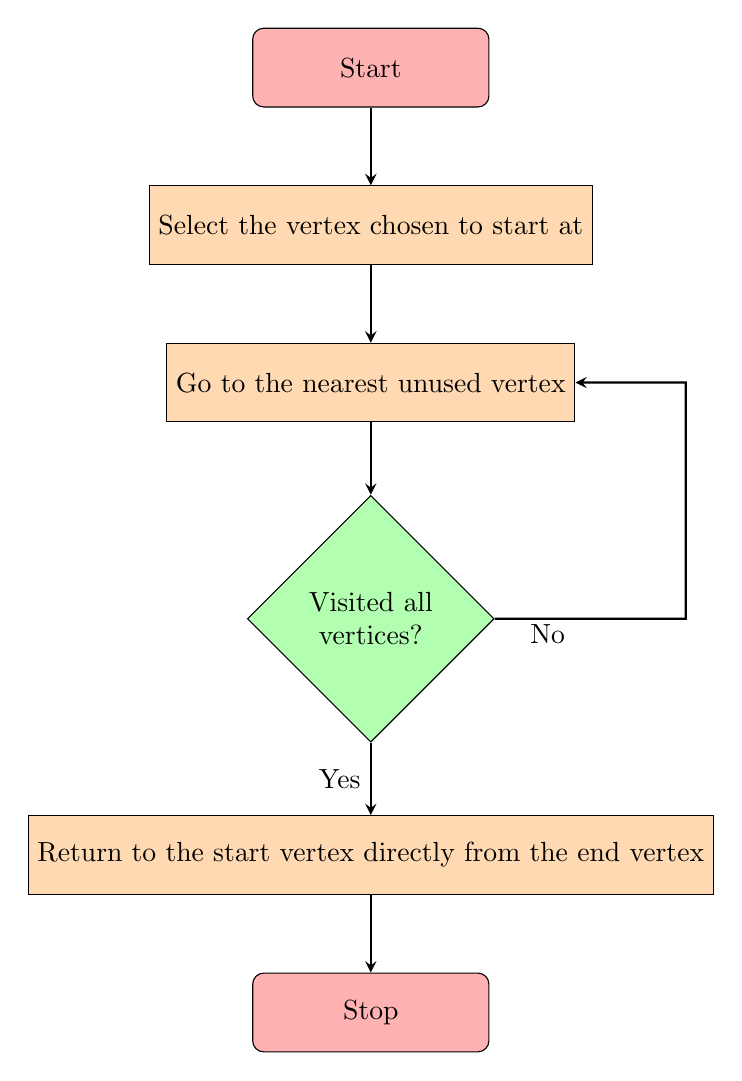
\begin{tikzpicture}[node distance=2cm]
\node (start) [startstop] {Start};
\node (pro1) [process, below of=start] {Select the vertex chosen to start at};
\node (pro2) [process, below of=pro1] {Go to the nearest unused vertex};
\node (dec1) [decision, below of=pro2, yshift=-1cm] {Visited all vertices?};
\node (pro3) [process, below of=dec1,yshift=-1cm] {Return to the start vertex directly from the end vertex};
\node (stop) [startstop,below of=pro3] {Stop};

\draw [arrow] (start) -- (pro1);
\draw [arrow] (pro1) -- (pro2);
\draw [arrow] (pro2) -- (dec1);
\draw [arrow] (pro3) -- (stop);
\draw [arrow] (dec1) -- node[anchor=east] {Yes} (pro3);
\draw [arrow] (dec1.east)  -- (4,-7) |- (pro2.east) node[anchor=east,yshift=-3.2cm] {No};





\end{tikzpicture}




\end{document}
